%% LaTeX2e class for student theses
%% sections/content.tex
%%
%% Karlsruhe University of Applied Sciences
%% Faculty of  Computer Science and Business Information Systems
%% Distributed Systems (vsys)
%%
%% Prof. Dr. Christian Zirpins
%% christian.zirpins@hs-karlsruhe.de
%%
%%
%% Version 0.2, 2017-11-15
%%
%% --------------------------------------------------------
%% | Derived from sdqthesis by Erik Burger burger@kit.edu |
%% --------------------------------------------------------

\chapter{Grundlagen zur sicheren Umsetzung dezentraler sozialer Netzwerke}
\label{ch:fundamentals}

\section{ActivityPub Standard}
	ActivityPub definiert zwei Protokollschichten, sowie Konzepte, Sammlungen und Interaktionen für dezentrale soziale Netzwerke. Es setzt auf bereits bestehenden Empfehlungen des W3C auf, welche teilweise auch von der SWWG entwickelt wurden wie zB. Activity Streams Core und Activity Streams Vocab. 
	\\\\Auch andere Technologien wie JSON-LD\footnote{\url{https://www.w3.org/TR/json-ld/}} werden benutzt um die Erweiterbarkeit zu gewährleisten. Über neue Ontologien (Vokabulare) können weitere syntaktische Definitionen und semantische Beschreibungen zu den bestehenden hinzugefügt werden. Diese Vokabulare können im Kontext des JSON-LD Objektes angegeben werden.\\ 
	\textbf{(Stimmt das mit den Ontologien???)}
		\textbf{(Beispiel Context Abbildung mit erweitertem Context???)}

\subsection{Bestandteile des Protokolls}
	Im Grunde besteht der ActivityPub Standard aus zwei Protokollen:
	\begin{itemize}
		\item ActivityPub Client-zu-Server Protokoll (Social API)
		\item ActivityPub verteiltes Server-zu-Server Protokoll (Federation Protocol)
	\end{itemize}
	Die beiden Protokolle können unabhängig voneinander implementiert werden. Das Client-zu-Server Protokoll besteht aus einem Client und Server Teil.
	\\\\ In ActivityPub werden Benutzer als \glqq Aktoren\grqq(actors) dargestellt. Jedes Aktoren Objekt muss eine \glqq Inbox\grqq~und \glqq Outbox\grqq, welche geordnete Sammlungen sein müssen, sowie eine ID und ein Typ besitzen\footnote{\href{https://www.w3.org/TR/activitypub/}{actor-objects https://www.w3.org/TR/activitypub/}}. Die ID muss global einzigartig sein und der Typ kann variieren zwischen \glqq Person\grqq, \glqq Application\grqq~und weiteren.\footnote{\href{https://www.w3.org/TR/activitystreams-core/}{actors https://www.w3.org/TR/activitystreams-core/}}
	
	\lstinputlisting[caption={Beispiel Aktoren Objekt}, label=listing::actor, language=JavaScript]{resources/mastodon-macu.json}

\subsection{Zugehörige Standards}
	ActivityPub benutzt die ActivityStream Daten Syntax und das Vokabular. Zusätzlich kann das Sicherheitsvokabular von Webpayments benutzt werden um Syntax und Semantik für das Beschreiben eines öffentlichen Schlüssels o.ä. zur Verfügung zu stellen.

\section{Client-zu-Server Kommunikation}
	
	Der Client empfängt Nachrichten über zwei Schnittstellen. Er kann sich per HTTP GET Anfrage auf seine eigene \glqq Inbox\grqq~die neusten an ihn adressierten Inhalt holen. Außerdem kann eine HTTP GET Anfrage an die \glqq shared Inbox\grqq~des Servers gesendet werden um eine Repräsentation aller Inhalte der Instanz zu bekommen.\\ \textbf{(Oder alle Inhalte des bekannten Netzwerks???)}\\\\
	\begin{figure}[h]
		\centering
		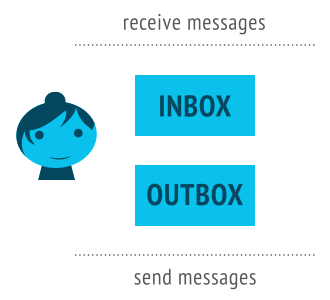
\includegraphics[scale=0.6]{figures/inbox-outbox.png}
		\label{Client zu Server Interaktionen}
		\caption{Interaktionen des Client mit dem Server}
	\end{figure}\\
	Um neue Aktivitäten an seine Folgenden, direkt an einzelne Personen oder sichtbar innerhalb der Domain zu veröffentlichen kann der Client eine HTTP POST Anfrage an seine \glqq Outbox\grqq~senden mit einer Aktivität oder einem ActivityStreams 2.0(AS2) Objekt als Inhalt. 
	

	\subsection{Client Teil}
		%%The client, represented as an actor, interacts with the server in two ways. First through sending a HTTP GET request with an Activity object to an actors inbox and through HTTP POST an Activity object to an actors outbox. An inbox and outbox must be a OrderedCollection.
		Der Client Teil des Client-zu-Server Protokolls beinhaltet mehrere Aufgaben:
		\begin{itemize}
			\item Auffinden der URL über das Profil
			\item Serialisieren der Daten in eine Aktivität oder AS2 Objekt
			\item Adressieren von Aktivitäten oder AS2 Objekten
			\item Eine HTTP POST Anfrage mit \glqq Content-Type: application/ld+json: profile="https://w3.org/ns/activitystreams"\grqq~oder \glqq Content-Type: application/activity+json: profile="https://w3.org/ns/activitystreams"\grqq~an seine \glqq Outboxg\grqq~absetzen
			\item Bei den Aktivitätstypen CREATE, UPDATE, DELETE, FOLLOW, ADD, REMOVE, LIKE, BLOCK, UNDO wird die \glqq object\grqq~Eigenschaft bereitgestellt
			\item Die \glqq target\grqq~Eigenschaft wird bei den Aktivitätstypen ADD und REMOVE bereitgestellt
			\item Anfragen müssen mit den Zugangsdaten des Nutzer, zu dem die \glqq Outbox\grqq~gehört, authentifiziert werden
		\end{itemize}
		Zusammengefasst muss sich der Client um das Entdecken von Endpunkten - Inbox/Outbox - über Profile, das Serialisieren von Daten zu Aktivitäten oder AS2 Objekten sowie um das setzen der entsprechenden Kopfzeilen (Mittlerer Teil der obigen Auflistung) und absenden der HTTP POST Anfrage kümmern. Außerdem muss bei HTTP GET Anfragen an den Server die \glqq ACCEPT: application/ld+json\grqq Kopfzeile gesetzt sein.
		
	\subsection{Server Teil}
  		Zu den Aufgaben des Serverteils gehören das Annehmen von HTTP POST Anfragen auf die \glqq Outbox\grqq~eines Nutzers und das verifizieren ob der Nutzer berechtigt ist diese Anfrage zu tätigen. Weiter werden die \glqq Inbox\grqq~Endpunkte bereitgestellt um authentifizierten Nutzern den Zugriff auf die neusten Inhalte zu geben.
  		\\\\
  		\textbf{(Ist das richtig oder bestehen die Aufgaben des Serverteils auch im weiterleiten zu anderen Instanzen, weil das ist ja eigentlich der Server-zu-Server Teil???) (Ist der Server Teil ein interner Speicher Mechanismus der Instanz oder ein delivery Mechanismus für alle Instanzen des Netzwerk oder für alle Instanzen mit einer Federated Implementierung insgesamt??? Ich verstehe es wie oben beschrieben, also ohne Server-to-Server Teil alles innerhalb einer Instanz)
  		\\\\
  		Angenommen der Server Part beinhaltet nicht nur das annehmen und abspeichern innerhalb einer Instanz, sonder auch das weiterleiten an andere Instanzen:
  		\\\\
  		Dann müsste ein Nutzer alleine durch die Implementierung des Server Teils des Client-zu-Server Protokolls in der Lage sein Inhalt mit anderen Servern auszutauschen. Den Unterschied zu einem förderierten Server liegt dann im Empfangen von öffentlichen Nachrichten (5.6 Public Addressing | Shared Inbox Delivery \footnote{\href{https://www.w3.org/TR/activitypub/}{sharedInbox https://www.w3.org/TR/activitypub/}}) und dem Weiterleiten (7.1.2 Forwarding from Inbox) von auf dieser Domäne nicht zustellbaren Empfängern.\\\\ Im Endeffekt ist die Frage ob der Server Teil des Client-zu-Server Protokolls eine Teilmenge des Server-zu-Server Protokolls ist???}
\section{Server-zu-Server Kommunikation}
	\begin{figure}[h]
		\centering
		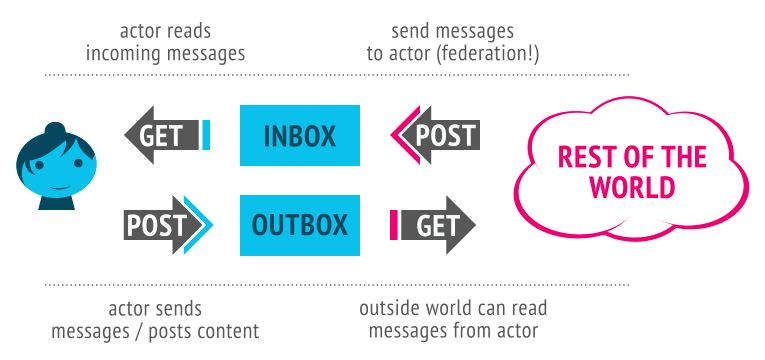
\includegraphics[scale=0.55]{figures/client-server-federated.png}
		\label{Client zu Server und Server zu Server Interaktionen}
		\caption{Schnittstellen des ActivityPub Protokolls}
	\end{figure}
Bei der Server-zu-Server Kommunikation bestehen die Hauptaufgaben im annehmen und zustellen von HTTP POST Anfragen auf die \glqq Inboxen\grqq~ und \glqq Outboxen\grqq~der Nutzer und im weiterleiten von Aktivitäten die der Server nicht zustellen kann. Dazu kommt das Bereitstellen der \glqq Outbox\grqq~Sammlungen.
\section{Authentifizierung und Datenintegrität}
	Für die Authentifizierung und zum sichern der Datenintegrität definiert der Standard keine Mechanismen. Es gibt allerdings \glqq Best Practices\grqq~für die Umsetzung dieser Anforderungen.
	\\\\Zum einen werden bei der Client-zu-Server Authentifizierung \glqq OAuth 2.0\grqq~Tokens benutzt, zum anderen auf der Server Seite HTTP Signaturen oder \glqq Linked Data Signatures\grqq zur Sicherstellung der Datenintegrität. Letztere Signatur wird eher verwenden wenn Objekte übertragen und weitergeleitet werden, da damit die Integrität des Objekts an sich verifiziert werden kann.\footnote{\url{https://www.w3.org/wiki/SocialCG/ActivityPub/Authentication_Authorization}}